% Set the author and title of the compiled pdf
\hypersetup{
	pdftitle = {\Title},
	pdfauthor = {\Author}
}

\section{Introduction}

We want computers to be able to interact with us, just like we interact with
them. This involves having them understand written text and voiced speech, as
well as being able to synthesise speech and text themselves. This includes
things like translation text and searching for key words in text.

A computer or a suite of programs that can do all of this is the goal for
Natural Language Systems. The catch is, that language is hard and complicated,
and to make computers do the things we want them to, we need to know how3
language works, and express this as an executable program.

Language is the representation of ideas, and the linkage of different ideas
together in such a way as to create new ideas. In order to understand any one
sentence (a sentence usually corresponds to one idea, event or action), we have
to understand what each symbol in the language means in isolation, and
understand how they're connected, and what the connections to do change the
meaning of the ideas.

Many factors affect the meaning of a sentence, but the connection between words
is always hierarchical, and we can represent sentences as trees:

\begin{figure}[ht]
  \centering
  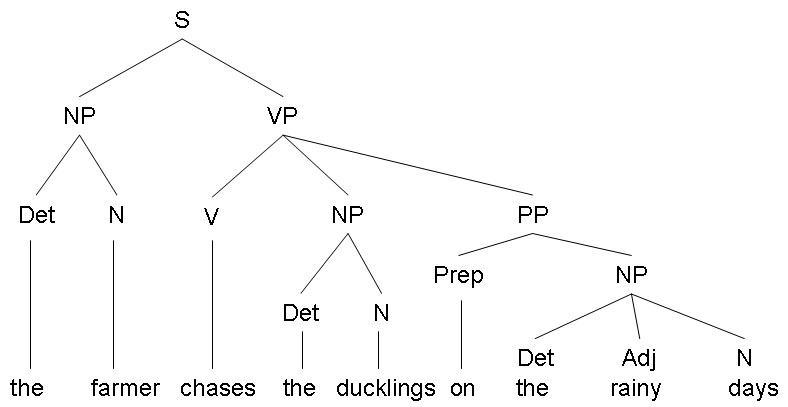
\includegraphics[width=0.55\textwidth]{images/phase-structure-tree}
  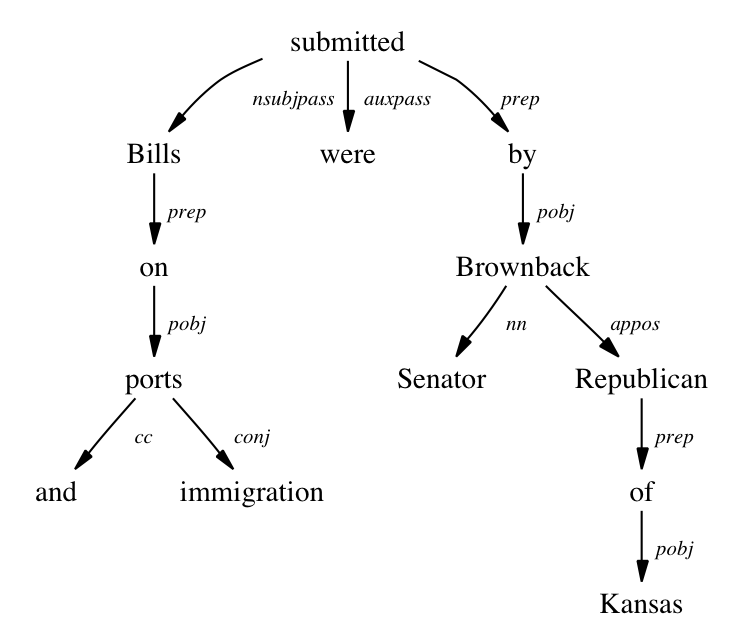
\includegraphics[width=0.35\textwidth]{images/dependency-tree}
  \caption{The left image is a phase structure tree, and the right image is a
  dependency tree.}
  \label{fig:trees}
\end{figure}

A parse tree is all well and good, but to a computer, this is only slightly more
useful than the original text. Though we have extracted some information out of
the text, we still just have a hierarchy of words, but we want a hierarchy of
ideas.

Having ideas instead of words allows us to infer more than what the text
literally says:

\begin{itemize}
  \item I'm fixing my motorbike $\rightarrow$ This person possesses a
  motorbike, and it is currently broken.
  \item The cake smells good $\rightarrow$ There is cake somewhere. Somebody is
  close enough to smell it.
\end{itemize}

But how can we do that?

\section{Structural analysis}

It is possibly to try and find out the meaning of a word simply by looking at
what letters it is made up of. One way to do this is to split a word into
\textbf{morphemes}, which are the most basic meaning-carrying components of a
word, and try to associate a meaning with each. For example \textit{undone}
could be split into \textit{un} and \textit{done}, and meaning associated with
each.

\subsection{Tries}

\marginpar{Tries are very handy datastructures for technical interviews, you
should read up on them an implement one!}

In order to examine the syntactic and semantic properties of the words, we need to represent them in the computer. A common way to do this is with a \textit{trie}:

\begin{wrapfigure}{r}{0.25\textwidth}
  \begin{center}
    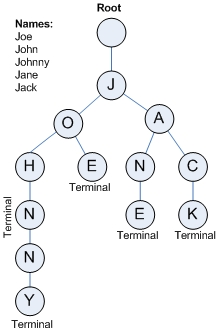
\includegraphics[width=0.24\textwidth,keepaspectratio]{images/trie}
  \end{center}
  \caption{A trie storing some names.}
\end{wrapfigure}

Tries are very memory efficient, since they if multiple words share the same
prefix, then the prefix is only stored once in memory. Tries have a lookup time
of $O(m)$, where $m$ is the length of the word, which is quite good, and is
better than a hash table in terms of speed in some cases. If you're stupid
enough to represent your dictionary as a list of words, then you can do a binary
search if its ordered (worst case $O(log(n) * m)$ comparisons (the $m$ comes
from having to possibly compare each character in the word)), or a linear search
if it isn't ordered ($O(m*n)$ in the worst case!).

\subsection{Spelling rules}

We want to understand why combining \textit{big} and \textit{est} produces
\textit{biggest} with an extra \textit{g}. Why isn't it \textit{bigest}? The
reason why we want to understand this, is so we can go from a word that we're
processing in text, and pick it apart into its components so we can better
understand it.

That is to say, we're going from \textit{biggest} to \textit{big} +
\textit{est}.

The format of the rules we're using in the course is as follows:

\marginpar{You can use \texttt{cX} and \texttt{vX} where \texttt{X} is an
integer, and \texttt{c/v} denotes a consonant or vowel inside the context
brackets.}

\begin{verbatim}
  [from] ==> [to]: [prevContext] _ [nextContext];
\end{verbatim}

For example, if we had a rule like:

\begin{verbatim}
  [g] ==> []: [g] _ [e,s,t];
\end{verbatim}

It would turn \textit{biggest} into \textit{big} + \textit{est}.
